\section{Administrative Information}

\begin{frame}\frametitle{Format}
\begin{blockitems}{Room}
\item lectures and exercises in person --- if we have a room
\item interaction strongly encouraged
 \lec{We don't want to lecture ---}
 \lec{we want to have a conversation during which you learn}
\item possibly make use of zoom
% \begin{itemize}
% \item use reactions to say yes no, ask for break etc.
% \item feel free to annotate my slides
% \item talk in the chat
% \end{itemize}
\end{blockitems}

\begin{blockitems}{Recordings}
\item maybe prerecorded video lectures or recorded zoom meeting
\item to be decided along the way
\end{blockitems}
\end{frame}


\begin{frame}\frametitle{Background}
\begin{blockitems}{Instructor}
\item PD Dr. Florian Rabe
\item Prof. Dr. Michael Kohlhase \lec{Professor of Knowledge Representation and Processing}
\end{blockitems}

\begin{blockitems}{Course}
\item This course is given for the fourth time
\item Still a bit experimental
  \lec{polishing and revising the materials this year}
\item Signature course of our research group \lec{same name!}
\end{blockitems}
\end{frame}

\begin{frame}\frametitle{Prerequisites}
\begin{blockitems}{Required}
\item basic knowledge about formal languages, context-free grammars
 \lec{but we'll do a quick revision here}
\end{blockitems}

\begin{blockitems}{Helpful}
\item Algorithms and Data Structures
 \lec{mostly as a contrast to this lecture}
\item Basic logic
 \lec{we'll revise it slightly differently here}
\item all other courses
 \lec{as examples of how knowledge pervades all of CS}
\end{blockitems}

\begin{blockitems}{General}
\item Curiosity \lec{this course is a bit unusual}
\item Interest in big picture \lec{this course touches on lots of things from all over CS}
\end{blockitems}
\end{frame}

\begin{frame}\frametitle{Examination and Grading}
\begin{blockitems}{Suggestion}
\item grade determined by single exam
\item probably written, 90 minutes
\item exercises indirectly graded through conversation during exam
\end{blockitems}
\lec{unless we agree on something else by the second week}

\begin{blockitems}{Exam-relevant}
\item anything mentioned in notes
\item anything discussed in lectures
\item anything done in exercises
\end{blockitems}
\lec{none is a superset of another!}
\end{frame}

\begin{frame}\frametitle{Materials and Exam-Relevance}
\begin{blockitems}{Textbook}
\item does not exist
\item normal for research-near specialization courses
\end{blockitems}

\begin{blockitems}{Notes}
\item textbook-style but not as comprehensive
\item developed along the way
\item systematic write-up, not necessarily in lecture order
\end{blockitems}

\begin{blockitems}{Slides}
\item not comprehensive
\item used as visual aid, conversation starters
\end{blockitems}
\end{frame}

\begin{frame}\frametitle{Communication}
\begin{blockitems}{Open for questions}
\item open door policy in our offices
\item always room for questions during lectures
\item for personal questions, contact me during/after lecture
\item matrix channel \url{https://matrix.to/\#/\#wuv:fau.de}
\item studon forum not used
\end{blockitems}

\begin{blockitems}{Materials}
\item notes and slides are at: \url{https://github.com/florian-rabe/Teaching/tree/master/WuV}
\item currently last year's version, will change throughout the semester
\lec{you can read ahead, but maybe don't print everything right away}
\item pull requests and issues welcome
\end{blockitems}
\end{frame}

\begin{frame}\frametitle{Exercises}
\begin{blockitems}{Learning Goals}
\item Get acquainted with state of the art of practice
\item Try out real tools
\end{blockitems}

\begin{blockitems}{Homeworks}
\item one major project as running example
\item homeworks building on each other
\end{blockitems}
\lec{build one large knowledge-based system}
\lec{details on later slides}
\end{frame}

\section{Overview and Essential Concepts}

\begin{frame}\frametitle{Representation and Processing}
Common pairs of concepts:
\begin{center}
\begin{tabular}{l|l}
Representation & Processing \\
\hline
Static & Dynamic \\
Situation & Change \\
Be & Become \\
Data Structures & Algorithms \\
Set & Function \\
State & Transition \\
Space & Time
\end{tabular}
\end{center}
\end{frame}

\begin{frame}\frametitle{Data and Knowledge}
$2\times 2$ key concepts
\begin{center}
\begin{tabular}{l|l}
Syntax & Data \\
\hline
Semantics & Knowledge
\end{tabular}
\end{center}

\begin{itemize}
\item Data: any object that can be stored in a computer\\
 Example: $((49.5739143, 11.0264941), "2020-04-21T16:15:00CEST")$
\item Syntax: a system of rules that describes which data is \textbf{well-formed}\\
 Example: ``a pair of (a pair of two IEEE double precision floating point numbers) and a string encoding of a time stamp''
\item Semantics: system of rules that determines the meaning of well-formed data
\item Knowledge: combination of some data with its syntax and semantics
\end{itemize}
\end{frame}

\begin{frame}\frametitle{Knowledge is Elusive}
Representation of key concepts 
\begin{itemize}
 \item Data: using primitive objects
  \lec{implemented as bits, bytes, strings, records, arrays, \ldots}
 \item Syntax: (context-free) grammars, (context-sensitive) type systems
  \lec{implemented as inductive data structures}
 \item Semantics: functions for evaluation, interpretation, of well-formed data
  \lec{implemented as recursive algorithms on the syntax}
 \item Knowledge: elusive
  \lec{emerges from applying and interacting with the semantics}
\end{itemize}
\end{frame}

\begin{frame}\frametitle{Semantics as Translation}
\begin{itemize}
\item Knowledge can be captured by a higher layer of syntax
\item Then semantics is translation into syntax
\end{itemize}

\begin{center}
\begin{tabular}{l|l|l}
Data syntax & Semantics function & Knowledge syntax \\
\hline
SPARQL query & evaluation & result set \\
SQL query & evaluation & result table \\
program & compiler & binary code \\
program expression & interpreter & result value \\ 
logical formula & interpretation in a model & mathematical object \\
HTML document & rendering & graphics context
\end{tabular}
\end{center}
\end{frame}

\begin{frame}\frametitle{Heterogeneity of Data and Knowledge}
\begin{itemize}
\item Capturing knowledge is difficult
\item Many different approaches to semantics
 \begin{itemize}
  \item fundamental formal and methodological differences
  \item often captured in different fields, conferences, courses, languages, tools
 \end{itemize}
\item Data formats equally heterogeneous
 \begin{itemize}
 \item ontologies
 \item programs
 \item logical proofs
 \item databases
 \item documents
 \end{itemize}
\end{itemize}
\end{frame}

\begin{frame}\frametitle{Challenges of Heterogeneity}
\begin{blockitems}{Challenges}
\item collaboration across communities
\item translation across languages
\item conversion between data formats
\item interoperability across tools
\end{blockitems}

\begin{blockitems}{Sources of problems}
\item interoperability across formats/tools major source of
 \begin{itemize}
 \item complexity
 \item bugs
 \end{itemize}
\item friction in project team due to differing preferences, expertise
\item difficult choice between languages/tools with competing advantages
\begin{itemize}
 \item reverting choices difficult, costly
 \item maintaining legacy choices increases complexity
\end{itemize}
\end{blockitems}
\end{frame}

\begin{frame}\frametitle{Aspects of Knowledge}
\begin{itemize}
\item Tetrapod model of knowledge
  \lec{active research by our group}
\item classifies approaches to knowledge into five aspects
\end{itemize}

\begin{center}
\begin{tabular}{lll}
Aspect & KRLs (examples) & KPTs (examples) \\
\hline
ontologization & ontology languages (OWL), description logics (ALC) & reasoners, SPARQL engines (Virtuoso) \\
concretization & relational databases (SQL, JSON) & databases (MySQL, MongoDb) \\
computation & programming languages (C) & interpreters, compilers (gcc) \\
deduction & logics (HOL) & theorem provers (Isabelle) \\
narration & document languages (HTML, LaTeX) & editors, viewers
\end{tabular}
\end{center}
\end{frame}

\begin{frame}\frametitle{Relations between the Aspects}
Ontology is distinguished: capture the knowledge that the other four aspects share

\begin{center}
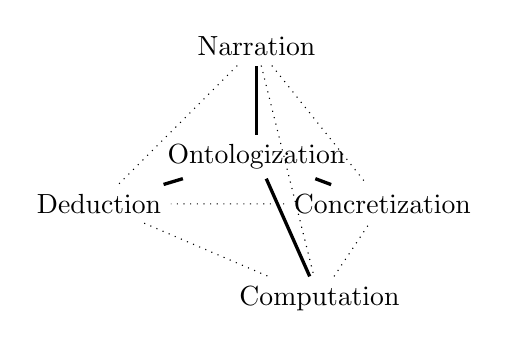
\begin{tikzpicture}[scale=4]
  \node (center) at (0,.15) {Ontologization};
  \node (left) at (.2,-.3) {Computation};
  \node (right) at (.4,0) {Concretization};
  \node (back) at (-.5,0) {Deduction};
  \node (up) at (0,.5) {Narration};

  \draw[very thick] (center) -- (left);
  \draw[very thick] (center) -- (right);
  \draw[very thick] (center) -- (back);
  \draw[very thick] (center) -- (up);
  \draw[dotted] (left) -- (right) -- (back) -- (left);
  \draw[dotted] (up) -- (left);
  \draw[dotted] (up) -- (right);
  \draw[dotted] (up) -- (back);
\end{tikzpicture}
\end{center}
\end{frame}

\begin{frame}\frametitle{Complementary Advantages of the Aspects}
\begin{center}
\footnotesize
\begin{tabular}{|l|llp{2.1cm}l|}\hline
Aspect & objects & \multicolumn{3}{c|}{characteristic} \\
       &         & advantage & joint advantage of the other aspects & application \\\hline
ded. & formal proofs & correctness & ease of use & verification \\
comp. & programs & efficiency & well-definedness & execution\\
concr. & concrete objects & queriability & abstraction & storage/retrieval\\
narr. & texts & flexibility & formal semantics & human understanding\\\hline
\end{tabular}
\medskip

\begin{tabular}{|l|l|}\hline
Aspect pair & characteristic advantage \\\hline
ded./comp.  & rich meta-theory \\
narr./conc. & simple languages \\\hline
ded./narr.  & theorems and proofs \\
comp./conc. & normalization \\\hline
ded./conc.  & decidable well-definedness \\
comp./narr. & Turing completeness \\\hline
\end{tabular}
\end{center}
\end{frame}

\begin{frame}\frametitle{Structure of the Course}
\begin{blockitems}{Aspect-independent parts}
\item shared characteristics
\item general methods
\end{blockitems}

\begin{blockitems}{Aspects-specific parts}
\item one part for each aspect
\item high-level overview of state of the art
\item focus on comparison/evaluation of the aspect-specific results
\end{blockitems}
\end{frame}

\begin{frame}\frametitle{Structure of the Exercises}
\begin{blockitems}{One major project}
\item representative for a project that a CS graduate might be put in charge of
\item challenging heterogeneous data and knowledge
\item requires integrating/combining different languages, tools
\end{blockitems}
\lec{unique opportunity in this course because knowledge is everywhere}

\begin{blockitems}{Concrete project}
\item develop a campo/studnon-style KRP system for a university
\item lots of heterogeneous knowledge
 \begin{itemize}
 \item course and program descriptions
 \item legal texts
 \item websites
 \item grade tables
 \item code to generate diplomas
 \end{itemize} 
\item build a functional system applying the lessons of the course
\lec{we'll see how far we get --- priority is learning}
\end{blockitems}
\end{frame}
